\documentclass[12pt,letterpaper]{article}
\usepackage[utf8]{inputenc}
\usepackage[english]{babel}
\usepackage{listings}
\usepackage{xcolor}
\usepackage{graphicx}

%For syntax highlighting
\definecolor{codegreen}{rgb}{0,0.6,0}
\definecolor{codegray}{rgb}{0.5,0.5,0.5}
\definecolor{codepurple}{rgb}{0.58,0,0.82}
\definecolor{backcolour}{rgb}{1,1,1}

%%Sets different parameters
\lstdefinestyle{mystyle}{
	backgroundcolor=\color{backcolour},   
    commentstyle=\color{codegreen},
    keywordstyle=\color{magenta},
    numberstyle=\tiny\color{codegray},
    stringstyle=\color{codepurple},
    basicstyle=\ttfamily\footnotesize,
    breakatwhitespace=false,         
    breaklines=true,                 
    captionpos=b,                    
    keepspaces=true,                 
    numbers=left,                    
    numbersep=5pt,                  
    showspaces=false,                
    showstringspaces=false,
    showtabs=false,                  
    tabsize=4
}
\lstset{style=mystyle}

\title{\textbf{Department of Computer Science and Engineering}}
\author{\textbf{S.G.Shivanirudh , 185001146, Semester VI }}

\date{22 April 2021}

\begin{document}
\maketitle
\hrule
\section*{\center{UCS1601 - Internet Programming}}
\hrule 
\bigskip\bigskip

%Assignment name
\subsection*{\center{\textbf{Assignment 7: Website for InternationalConference using React}}}

%Objective
\subsection*{\flushleft{Objective:}}
\begin{flushleft}
    Design a Website for an International Conference using React.
\end{flushleft}

%Code
\subsection*{\flushleft{Code:}}
\subsubsection*{\flushleft{HTML:}}
\begin{flushleft}
\lstinputlisting[language = HTML]{website/public/index.html}
\end{flushleft}

\subsubsection*{\flushleft{Javascript:}}
\subsubsection*{\flushleft{App}}
\begin{flushleft}
\lstinputlisting{website/src/App.js}
\end{flushleft}

\subsubsection*{\flushleft{Home}}
\begin{flushleft}
\lstinputlisting{website/src/components/Home.js}
\end{flushleft}

\subsubsection*{\flushleft{Committee}}
\begin{flushleft}
\lstinputlisting{website/src/components/Committee.js}
\end{flushleft}

\subsubsection*{\flushleft{Papers}}
\begin{flushleft}
\lstinputlisting{website/src/components/Paper.js}
\end{flushleft}

\subsubsection*{\flushleft{Dates}}
\begin{flushleft}
\lstinputlisting{website/src/components/Dates.js}
\end{flushleft}

\subsubsection*{\flushleft{Workshop}}
\begin{flushleft}
\lstinputlisting{website/src/components/Workshop.js}
\end{flushleft}

\subsubsection*{\flushleft{Registration}}
\begin{flushleft}
\lstinputlisting{website/src/components/Registration.js}
\end{flushleft}

\subsubsection*{\flushleft{Contact}}
\begin{flushleft}
\lstinputlisting{website/src/components/Contact.js}
\end{flushleft}



\newpage
%Output
\subsection*{\flushleft{Output:}}
\subsubsection*{\flushleft{Home}}
\begin{figure}[h]
    \centering
    
\includegraphics[width = \textwidth]{Pics/home.png}
\end{figure}

\newpage
\subsubsection*{\flushleft{Committee}}
\begin{figure}[h]
    \centering
    
\includegraphics[width = \textwidth]{Pics/committee.png}
\end{figure}

\newpage
\subsubsection*{\flushleft{Papers}}
\begin{figure}[h]
    \centering
    
\includegraphics[width = \textwidth]{Pics/paper.png}
\end{figure}

\newpage
\subsubsection*{\flushleft{Dates}}
\begin{figure}[h]
    \centering
    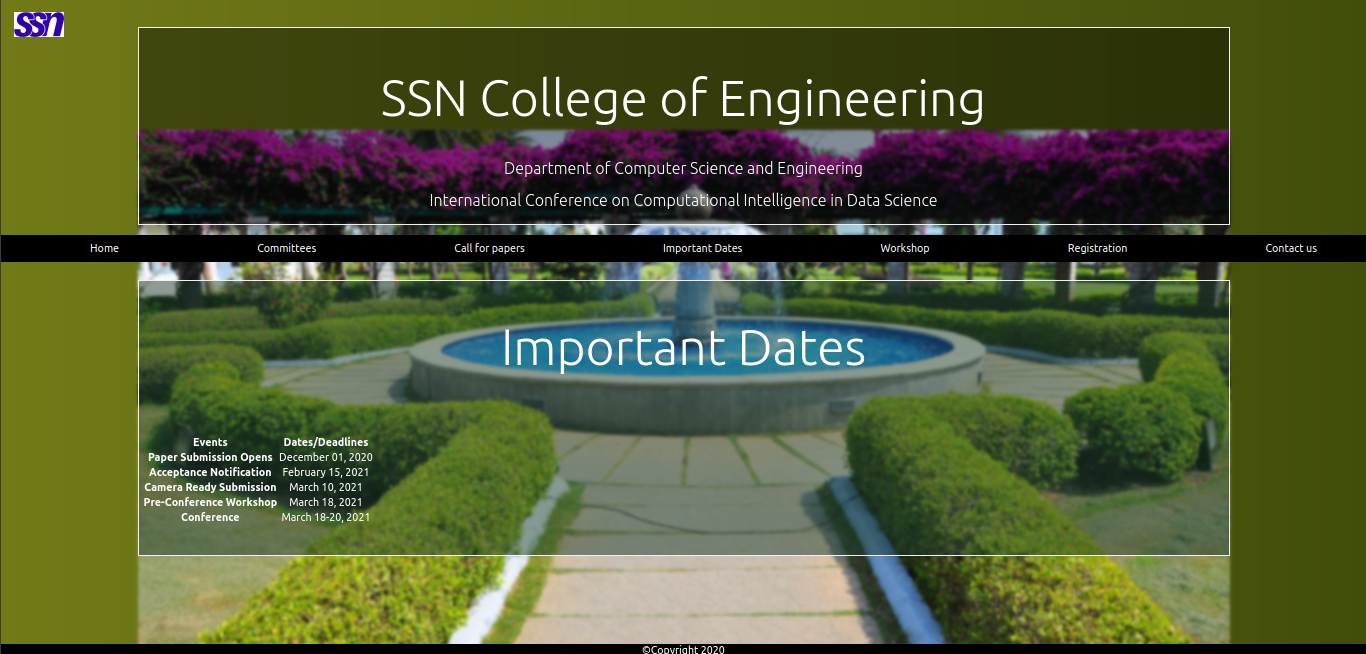
\includegraphics[width = \textwidth]{Pics/dates.png}
\end{figure}

\newpage
\subsubsection*{\flushleft{Workshop}}
\begin{figure}[h]
    \centering
    
\includegraphics[width = \textwidth]{Pics/workshop.png}
\end{figure}

\newpage
\subsubsection*{\flushleft{Registration}}
\begin{figure}[h]
    \centering
    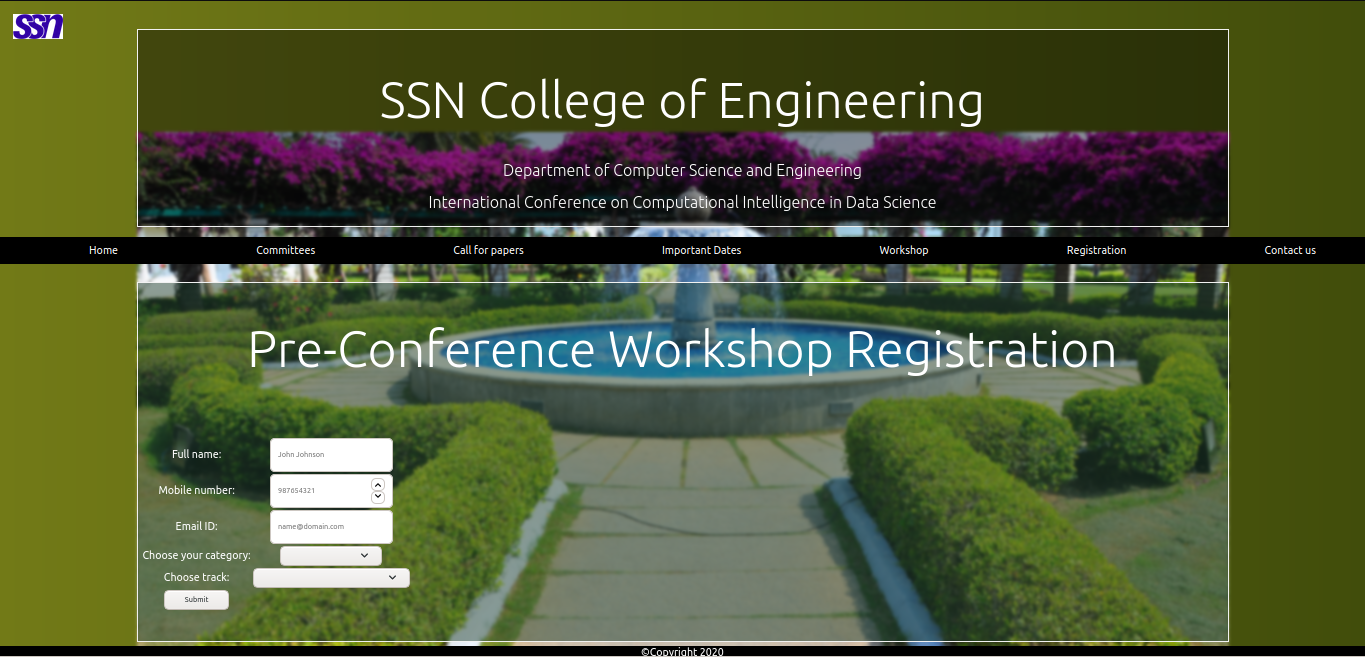
\includegraphics[width = \textwidth]{Pics/registration.png}
\end{figure}

\newpage
\subsubsection*{\flushleft{Contact}}
\begin{figure}[h]
    \centering
    
\includegraphics[width = \textwidth]{Pics/contact.png}
\end{figure}

\hrule
\end{document}